\documentclass[a4paper,12pt]{article}


%%% Работа с русским языком
\usepackage{cmap}					          % поиск в PDF
\usepackage[T2A]{fontenc}			      % кодировка
\usepackage[utf8]{inputenc}               % кодировка исходного текста
\usepackage[english, russian]{babel}   % локализация и переносы


%%% Страница 
\usepackage{extsizes} % Возможность сделать 14-й шрифт
\usepackage{geometry}  
\geometry{left=20mm,right=20mm,top=25mm,bottom=30mm} % задание полей текста

\usepackage{titleps}      % колонтитулы
\newpagestyle{main}{
	\setheadrule{.4pt}                      
	\sethead{\CourseName}{}{\hyperlink{intro}{\;Назад к содержанию}}
	\setfootrule{.4pt}                       
	\setfoot{\CourseDate \; ФПМИ МФТИ}{}{\thepage} 
}      
\pagestyle{main}    % Устанавливает контитулы на странице


%%%  Текст
\setlength\parindent{0pt}         % Устанавливает длину красной строки 0pt
\sloppy                                        % строго соблюдать границы текста
\linespread{1.3}                           % коэффициент межстрочного интервала
\setlength{\parskip}{0.5em}                % вертик. интервал между абзацами
%\setcounter{secnumdepth}{0}                % отключение нумерации разделов
%\setcounter{section}{-1}         % Чтобы сделать нумерацию лекций с нуля
\usepackage{multicol}				          % Для текста в нескольких колонках
%\usepackage{soul}
\usepackage{soulutf8} % Модификаторы начертания


%%% Гиппер ссылки
\usepackage{hyperref}
\usepackage[usenames,dvipsnames,svgnames,table,rgb]{xcolor}
\hypersetup{				% Гиперссылки
	unicode=true,           % русские буквы в раздела PDF\\
	pdfstartview=FitH,
	pdftitle={Заголовок},   % Заголовок
	pdfauthor={Автор},      % Автор
	pdfsubject={Тема},      % Тема
	pdfcreator={Создатель}, % Создатель
	pdfproducer={Производитель}, % Производитель
	pdfkeywords={keyword1} {key2} {key3}, % Ключевые слова
	colorlinks=true,       	% false: ссылки в рамках; true: цветные ссылки
	linkcolor=blue,          % внутренние ссылки
	citecolor=green,        % на библиографию
	filecolor=magenta,      % на файлы
	urlcolor=NavyBlue,           % на URL
}


%%% Для формул
\usepackage{amsmath}          
\usepackage{amssymb}


%%%%%% theorems
\usepackage{amsthm}  % for theoremstyle

\theoremstyle{plain} % Это стиль по умолчанию, его можно не переопределять.
\newtheorem{theorem}{Теорема}[section]
\newtheorem{prop}[theorem]{Утверждение}
\newtheorem{lemma}{Лемма}[section]
\newtheorem{sug}{Предположение}[section]

\theoremstyle{definition} % "Определение"
\newtheorem{Def}{Определение}
\newtheorem{corollary}{Следствие}[theorem]
\newtheorem{problem}{Задача}[section]

\theoremstyle{remark} % "Примечание"
\newtheorem*{nonum}{Решение}
\newtheorem*{definition}{Def}
\newtheorem*{example}{Пример}
\newtheorem*{note}{Замечание}


%%% Работа с картинками
\usepackage{graphicx}                           % Для вставки рисунков
\graphicspath{{images/}{images2/}}        % папки с картинками
\setlength\fboxsep{3pt}                    % Отступ рамки \fbox{} от рисунка
\setlength\fboxrule{1pt}                    % Толщина линий рамки \fbox{}
\usepackage{wrapfig}                     % Обтекание рисунков текстом
\graphicspath{{images/}}                     % Путь к папке с картинками

\newcommand{\drawsome}[1]{            % Для быстрой вставки картинок
    \begin{figure}[h!]
            \centering
            \includegraphics[scale=0.7]{#1}
            \label{fig:first}
    \end{figure}
}
\newcommand{\drawsomemedium}[1]{
    \begin{figure}[h!]
            \centering
            \includegraphics[scale=0.45]{#1}
            \label{fig:first}
    \end{figure}
}
\newcommand{\drawsomesmall}[1]{
    \begin{figure}[h!]
            \centering
            \includegraphics[scale=0.3]{#1}
            \label{fig:first}
    \end{figure}
}

\definecolor{faded}{gray}{0.8}

%%% Вставка кусков кода:

%% Код вставляется в окружение lstisting

%\usepackage{xcolor} % для выделений и прочих использований цветов
%
%\usepackage{listings}
%\lstset{ 
%  backgroundcolor=\color{white},   % цвет фона
%  basicstyle=\footnotesize,        % размер
%  breakatwhitespace=false,         % проблемы с отступами
%  breaklines=true,                 % автоматический переход на новую строку
%  captionpos=b,                    % sets the caption-position to bottom
%  commentstyle=\color{black},      % стиль комментариев
%  escapeinside={\%*}{*)},          % для вставки латеха в код
%  frame=single,	                   % рамочка вокруг
%  keepspaces=true,                 % сохраняет пробелы в коде (чтобы был кодстайл)
%  keywordstyle=\color{blue},       % стиль кода
%  language=C++,                    % язык программирования!
%  morekeywords={*,...},            % увеличение словаря
%  numbers=left,                    % где будет нумерация строк (none, left, right)
%  numbersep=8pt,                   % расстояние между нумерацией и кодом
%  numberstyle=\color{gray},        % стиль нумерации
%  rulecolor=\color{gray},          % цвет рамки
%  showspaces=false,                % если тру, то заменяет пробелы на особые подчеркивания; конфликтует с 'showstringspaces'
%  showstringspaces=false,          % особые подчеркивания вместо пробелов в строках
%  showtabs=false,                  % подчеркивания вместо табов
%  stepnumber=1,                    % как часто показывать нумерацию. Если 1, то нумеруется каждая строка
%  stringstyle=\color{violet},      % цвет строк
%  tabsize=2,	                       % дефолтный размер таба
%  texcl=true,
%  title=\lstname                   % вставляет название файла, если импорт
%}



%%% облегчение математических обозначений
\newcommand{\R}{\mathbb{R}}
\newcommand{\N}{\mathbb{N}}
%\newcommand{\C}{\mathbb{C}}             % команда уже определена где-то)
\newcommand{\Z}{\mathbb{Z}}
\newcommand{\E}{\mathbb{E}}
\newcommand{\brackets}[1]{\left({#1}\right)}      % автоматический размер скобочек
% Здесь можно добавить ваши индивидуальные сокращения  

%% Приставки СИ
\newcommand{\sda}{\text{да}}
\renewcommand{\sh}{\text{г}}
\newcommand{\sk}{\text{к}}
\newcommand{\sM}{\text{М}}
\newcommand{\sG}{\text{Г}}
\newcommand{\sT}{\text{Т}}
\newcommand{\sP}{\text{П}}
\newcommand{\sE}{\text{Э}}
\newcommand{\sZ}{\text{З}}
\newcommand{\sY}{\text{И}}
\newcommand{\sd}{\text{д}}
\renewcommand{\sc}{\text{с}}
\newcommand{\sm}{\text{м}}
\newcommand{\smu}{\text{мк}}
\newcommand{\sn}{\text{н}}
\renewcommand{\sp}{\text{п}}
\renewcommand{\sf}{\text{ф}}
\newcommand{\sa}{\text{а}}
\newcommand{\sz}{\text{з}}
\newcommand{\sy}{\text{и}}

%% Базовые единицы СИ
\newcommand{\m}{\text{м}}
\newcommand{\kg}{\text{кг}}
\newcommand{\s}{\text{с}}
\newcommand{\A}{\text{А}}
\newcommand{\K}{\text{К}}
\newcommand{\mol}{\text{моль}}
\newcommand{\kd}{\text{кд}}

%% Некоторые производные единицы
% Механика
\newcommand{\hz}{\text{Гц}}
\newcommand{\cm}{\text{см}}
\newcommand{\mm}{\text{мм}}
\newcommand{\km}{\text{км}}
\newcommand{\g}{\text{г}}
\newcommand{\J}{\text{Дж}}
\newcommand{\erg}{\text{эрг}}

% Электромагнетизм
\newcommand{\V}{\text{В}}
\newcommand{\T}{\text{Тл}}
\renewcommand{\G}{\text{Гс}}
\newcommand{\Wb}{\text{Вб}}
\newcommand{\Oe}{\text{Э}}
\newcommand{\Ohm}{\text{Ом}}
\newcommand{\F}{\text{Ф}}
\renewcommand{\H}{\text{Гн}}



\newcommand{\CourseName}{Электричество и магнетизм} %  Используется в преамбуле для создания названия предмета в верхнем контитуле   
\newcommand{\CourseDate}{Осень 2020}           %  Используется в преамбуле для создания даты в нижнем контитуле и в title_page

%\includeonly{lectures/lect05,lectures/lect06}  % Чтобы скомпилировать только часть лекций

\begin{document}
    %%% Если будут вопросы по преамбуле, не стесняйтесь спрашивать

%%% Всю шаблонную информацию можно менять тут
\newcommand{\FullCourseNameFirstPart}{\so{ОБЩАЯ ФИЗИКА}}
\newcommand{\FullCourseNameSecondPart}{\so{Электричество и магнетизм}}
\newcommand{\SchoolName}{ФПМИ}
\newcommand{\TrackName}{ПМФ МФ}
\newcommand{\SemesterNumber}{III}
\newcommand{\LecturerInitials}{Аланакян Юрий Робертович}
\newcommand{\AutherInitials}{Зайцева Алла}
\newcommand{\VKLink}{https://vk.com/alla.zaytseva}
\newcommand{\GithubLink}{https://github.com/Alla-Zaitseva/Phyzics}

\begin{titlepage}
	\clearpage\thispagestyle{empty}
	\centering
	
	\textit{Федеральное государственное автономное учреждение \\
		высшего профессионального образования}
	\vspace{0.5ex}
	
	\textbf{Московский Физико-Технический Институт \\ КЛУБ ТЕХА ЛЕКЦИЙ}
	\vspace{20ex}
	
	\rule{\linewidth}{0.5mm}
	{\textbf{\FullCourseNameFirstPart}}
	\\
	{\textbf{\FullCourseNameSecondPart}}
	\rule{\linewidth}{0.5mm}
	
	\SemesterNumber\ СЕМЕСТР
	\\
	Физтех Школа: \textit{\SchoolName}
	\\
	Направление: \textit{\TrackName}
	\\
	Лектор: \textit{\LecturerInitials}
	\vspace{1ex}
	
	\begin{figure}[!ht]
		\centering
		
\includegraphics[width=0.4\textwidth]{logo_LTC.png}
		\label{fig:my_label}
	\end{figure}
\begin{flushright}
	\noindent
	Автор: \href{\VKLink}{\textit{\AutherInitials}}
	\\
	\href{\GithubLink}{\textit{Проект на github}} % Опционально, если хотите учавствовать в рейтинге
\end{flushright}
	
	\vfill
	\CourseDate\ года
	\pagebreak
	
\end{titlepage}

    \newpage
    \hypertarget{intro}{}
    \tableofcontents
    
    \newpage
\section{Лекция. Закон Кулона. Напряженность электрического поля. Диполь. Теорема Гаусса}
\subsection{Введение}
3 семестр будет посвящен электромагнитизму. Давайте зададимся вопросом, почему это важнейший раздел? Потому что все вокруг нас связано с электрическими и магнитными взаимодействиями. Даже давление на стол является электрическим взаимодействием. 

\textit{Исторический факт: о важности электромагнитных взаимодействий задумались всего пару веков назад.}

\large
\textbf{\textit{Демонстрация №1}}.\\
\normalsize
Если натереть эбонитовую палочку шерстью, то можно увидеть, что стрелка на электроскопе отклоняется. А если стекло натереть о шелк, то пстрелка отклоняется в другую сторону.\\
Таким образом, видно, что \underline{существует 2 типа зарядов} - \textbf{положительный и отрицательный}.

\colorbox{faded}{\underline{\textbf{Опр.}}} \textbf{Заряд} - способность частиц взаимодействовать между собой.

\textit{Многие студенты считают, что "отрицательный" это плохо, но это всего лишь название. В целом, отрицательными могли быть и протоны)}

В теоретической физике положительные и отрицательные заряды являются элементами симметрии. Так, с колоссальной точностью \underline{абсолютная величина заряда протона равна абсолютной величине заряда электрона.} Не менее важно, что если взять заряд какого-то тела и поделить на заряд электрона, то получится целое число. Другими словами можно сказать: \underline{заряд квантуется.}

\textbf{Важно!} 
$$e = 4,803*10^{-10} \text{ед.СГСЭ} = 1,602*10^{-19} \text{Кл}$$

\textit{Филосовское отступление: каким образом происходит притяжение положительного и отрицательного зарядов - пока не выявлено учёными. Во времена Ньютона считали, что между зарядами есть какая-то субстанция (эфир), но в последствии от данной идеи отказались.}

\newpage

\subsection{Закон Кулона}

Электромагнитные силы наблюдали еще до Шарля Кулона. Он же был первым, кто провел количественные измерения. Ученый создал крутильные весы, при помощи которых он измерил силу взаимодействия двух точечных зарядов. Так, в 1785 году был установлен закон Кулона.

\colorbox{faded}{\underline{\textbf{Закон Кулона}}} Сила взаимодействия между двумя зарядами $q_{1}$ и $q_{2}$ пропорциональна их произведению и обратно пропорциональна квадрату расстояния между ними: 

\begin{equation}\label{opr1}
\overline{F} = \frac{q_{1} q_{2}}{r^2} \frac{\overline{r}}{|\overline{r}|}
\end{equation}

\textit{Область применимости:} область применимости не обнаружена. Так про очень малых (ядерных) расстояниях также действует данный закон.

P.s. закон Кулона эквивалентен гравитационному закону.

\subsection{Напряженность электрического поля}

\colorbox{faded}{\underline{\textbf{Опр.}}} \textbf{Электрическое поле (ЭП)} - область пространства, где действуют электрические силы.

Пусть есть заряд \textit{q}. Вокруг него образуется электрическое поле. 

\colorbox{faded}{\underline{\textbf{Опр.}}} \textbf{Напряжённость ЭП в некоторой точке} - сила, действующая на единичный точечный заряд, помещенный в эту точку. Она равна:

\begin{equation}\label{opr2}
\overline{E} = \frac{q}{r^2} \frac{\overline{r}}{|\overline{r}|}
\end{equation}

\subsection{Принцип сукперпозиции}

Сила, действующая на заряд \textit{q} со стороны системы других зарядов, равна векторной сумме сил, независимо действующих на рассматриваемый заряд со стороны каждого из зарядов системы.

Поскольку $\overline{F_{i}} = q \overline{E_{i}}$, то напряженность поля в данной точке также равна векторной сумме напряженностей полей, независимо создаваемых в данной точке каждым из зарядов системы:

\begin{equation}\label{opr3}
\overline{E} = \sum\limits_{i=1}^n \overline{E_{i}}
\end{equation}

\begin{figure}[!ht]
\centering
 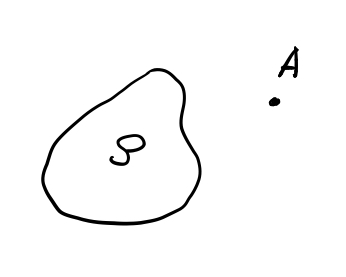
\includegraphics[width=0.4\textwidth]{1_1.jpg}     
 \label{fig:my_label}
 \caption{}
\end{figure}

Посмотрим на рисунок (1.1). Пустьестьнекоторый объем, где плотность заряда $\rho$. Это означает, что в точке \textit{A} поле, создаваемое всем зарядами:

\begin{equation}\label{opr4}
\overline{E_{A}} = \int \frac{\rho dV}{r^2} \frac{\overline{r}}{|\overline{r}|}
\end{equation}

\subsection{Электрический диполь}

\begin{figure}[!ht]
\centering
 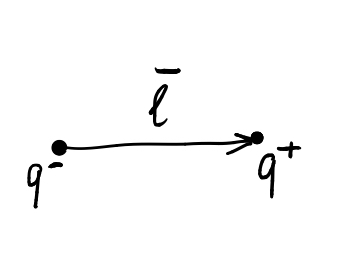
\includegraphics[width=0.4\textwidth]{1_2.jpg}     
 \label{fig:my_label}
 \caption{}
\end{figure}

\colorbox{faded}{\underline{\textbf{Опр.}}} \textbf{Диполь} - это система, состоящая из  двух одинаковых зарядов, одинаковых по величине и противоположных по знаку.

\colorbox{faded}{\underline{\textbf{Опр.}}} \textbf{Плечо диполя $\overline{l}$} - вектор, идущий от отрицательного заряда к положительному, длина которого равна расстоянию между зарядами.

\colorbox{faded}{\underline{\textbf{Опр.}}} \textbf{Дипольный момент} - вектор 

\begin{equation}\label{opr5}
\overline{p} =q \overline{l}
\end{equation}

\begin{figure}[!ht]
\centering
 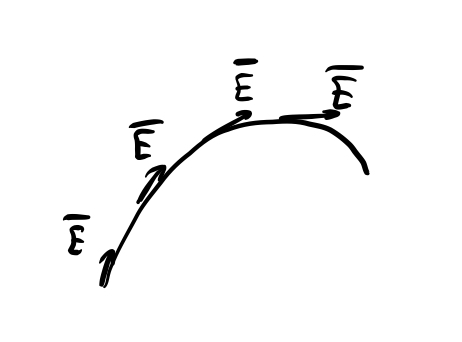
\includegraphics[width=0.4\textwidth]{1_3.jpg}     
 \label{fig:my_label}
 \caption{}
\end{figure}

\colorbox{faded}{\underline{\textbf{Опр.}}} \textbf{Cиловая линия} - линия, в каждой точке которой направление касательной совпадает с направлением напряжённости поля в той же точке. (смотри рис.3)

\colorbox{faded}{\underline{\textbf{Опр.}}} \textbf{Точечный диполь} - диполь, для которого выполнено: расстояние между его зарядами $l$ мало по сравнению с расстоянием $r$ от диполя до точки наблюдения: $l \ll r$

Найдем \underline{поле точечного диполя}:

$$\overline{E} = \frac{q}{r^2} \frac{\overline{r}}{|\overline{r}|} - \frac{q(\overline{r} + \overline{l})}{|\overline{r} + \overline{l}|^3}$$

Это выражение разложим в ряд Тейлора (трехмерное разложение):

\begin{equation}\label{opr6}
\overline{E} = \frac{3(\overline{p} \overline{r}) \overline{r}}{r^5} - \frac{\overline{p}}{r^3}
\end{equation}

\underline{Выведем формулу (6):}

\begin{figure}[!ht]
\centering
 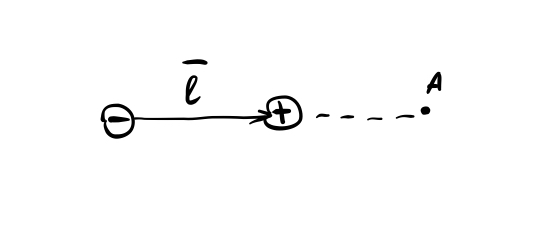
\includegraphics[width=0.4\textwidth]{1_4.jpg}     
 \label{fig:my_label}
 \caption{}
\end{figure}

1. Рассмотрим поле вдоль оси диполя (рисунок 4):
$$E = q \frac{d}{2} (\frac{1}{r^2}) l \Rightarrow \overline{E_{||}} = 2 \frac{\overline{p}}{r^3}$$

\begin{figure}[!ht]
\centering
 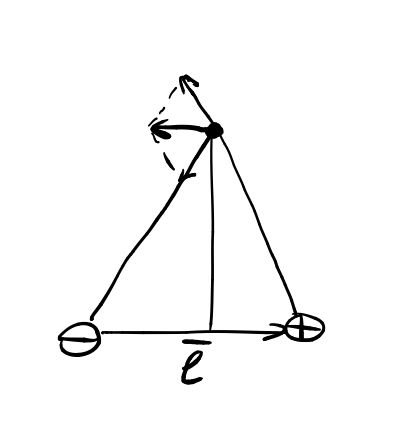
\includegraphics[width=0.4\textwidth]{1_5.jpg}     
 \label{fig:my_label}
 \caption{}
\end{figure}

2. Рассмотрим поле перпендекулярно оси диполя (рисунок 5):
$$\overline{E_{\perp}} =  \frac{q}{r^2} \frac{\overline{l}}{r}  \Rightarrow \overline{E_{\perp}} = - \frac{\overline{p}}{r^3}$$

В результате получим (рисунок 6):

\begin{figure}[!ht]
\centering
 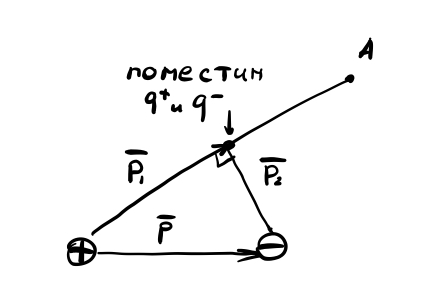
\includegraphics[width=0.4\textwidth]{1_6.jpg}     
 \label{fig:my_label}
 \caption{}
\end{figure}

$$ \overline{p}  = \overline{p_{1}} + \overline{p_{2}}$$
$$\Rightarrow \overline{E_{A}} = \frac{2p_{1} - p_{2}}{r^3}$$

Таким образом получили исходное уравнение (6).

\subsection{Демонстрации}

\large
\textbf{\textit{Демонстрация №2. "Манка -- это сила!"}}.\\
\normalsize
В данной демонстрации мы увидим диполь. Покажем его с помощью манной крупы. В каждой крупинке под действием ЭП заряды разделяются и каждая крупинка превращается в диполь. На экране видны 2 разноименных заряда. Включим ЭП.
Увидим, что крупинки рисуют силовые линии. 

\large
\textbf{\textit{Демонстрация №3. "Султанчики"}}.\\
\normalsize
Зарядим султанчики \underline{одноименно}. Тогда увидим что бумажные полоски расходятся. 
Зарядим султанчики \underline{разноименно}. Тогда увидим что бумажные полоски притягиваются.
\textit{Минутка юмора:} султанчики сходятся до свадьбы, а расходятся после) 

\subsection{Силы, действующие на диполь в ЭП}

\underline{Cлучай 1. $\overline{E} = const$}

\begin{figure}[!ht]
\centering
 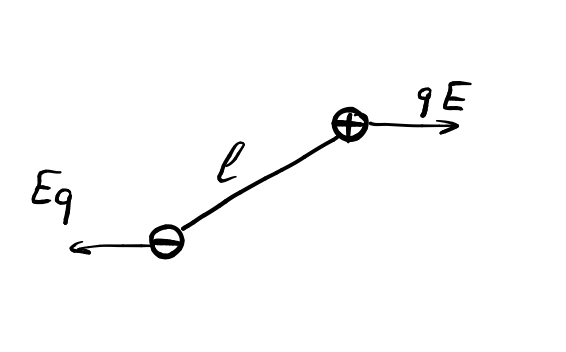
\includegraphics[width=0.4\textwidth]{1_7.jpg}     
 \label{fig:my_label}
 \caption{}
\end{figure}

Поместим диполь в ЭП (рис.7). Силы и напряжение указаны на рисунке. Суммарная сила равно 0, но возникает момент сил:

\begin{equation}\label{opr7}
\overline{N} = [\overline{l} \overline{F}] = [\overline{p} \overline{E}]
\end{equation}



\underline{Cлучай 2. $\overline{E} (\overline{r})$}

\begin{equation}\label{opr8}
F = \triangle x \frac{\partial \overline{E}}{\partial x} + \triangle y \frac{\partial \overline{E}}{\partial y} + \triangle z \frac{\partial \overline{E}}{\partial z}
\end{equation}

\colorbox{faded}{\underline{\textbf{Опр.}}} \textbf{Набла}:

\begin{equation}\label{opr9}
\nabla = \overline{i}  \frac{\partial}{\partial x} + \overline{j} \frac{\partial}{\partial y} + \overline{k} \frac{\partial}{\partial z}
\end{equation}

\colorbox{faded}{\underline{\textbf{Опр.}}} Когда оператор набла действует на скалярную функцию - получаем \textbf{градиент $\nabla \Phi$}.

Следовательно, преобразуем формулу (8):
\begin{equation}\label{opr10}
\overline{F} = (\overline{p} \nabla) \overline{E}
\end{equation}

\textbf{Важно:} диполь разворачивается и втягивается в область сильного поля.

\subsection{Теорема Гаусса}

\colorbox{faded}{\underline{\textbf{Опр.}}} \textbf{Поток вектора $d \text{Ф}$}: $d \text{Ф} = \overline{E} d \overline{S}$ поля \textit{Е} через площадь \textit{S}.

\colorbox{faded}{\underline{\textbf{Теорема Гаусса}}} Поток вектора \textit{Е} через замкнутую поверхность:

\begin{equation}\label{opr10}
  \oint \overline{E} d \overline{S} = 4 \pi q
\end{equation}

\underline{\textit{Доказательство:}}

\begin{figure}[!ht]
\centering
 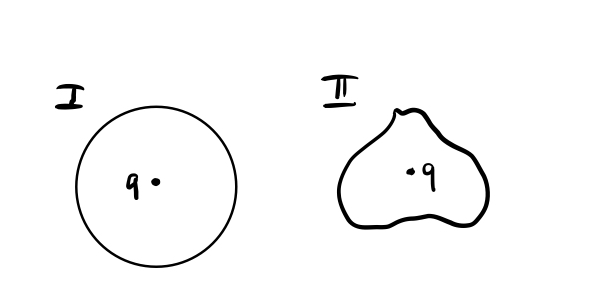
\includegraphics[width=0.4\textwidth]{1_8.jpg}     
 \label{fig:my_label}
 \caption{}
\end{figure}

\underline{Случай 1.} 
$$E = \frac{q}{r^2} \Rightarrow \text{Ф} = 4 \pi r^2 \frac{q}{r^2} = 4 \pi q$$

\underline{Случай 2.} 
$$\oint d \overline{S} \overline{E} = \oint \frac{q}{r^2}  d S = 4 \pi q
\Rightarrow d \Omega = \frac{\overline{r} d \overline{S}}{r^3} \text{-- элемент телесного угла}$$

\colorbox{faded}{\underline{\textbf{Теорема Иршоу}}} Невозможна устойчивая статическая конфигурация электрических зарядов

    \section{Лекция}

\end{document}